\documentclass[runningheads]{llncs}
%
\usepackage[T1]{fontenc}
% T1 fonts will be used to generate the final print and online PDFs,
% so please use T1 fonts in your manuscript whenever possible.
% Other font encondings may result in incorrect characters.
%
\usepackage{graphicx}
\usepackage{subcaption}
\usepackage{svg}
% Used for displaying a sample figure. If possible, figure files should
% be included in EPS format.
%
% If you use the hyperref package, please uncomment the following two lines
% to display URLs in blue roman font according to Springer's eBook style:
%\usepackage{color}
%\renewcommand\UrlFont{\color{blue}\rmfamily}
%\urlstyle{rm}
%
\begin{document}
%
\title{Exploring public space congestion via Bluetooth device counting}
%
%\titlerunning{Abbreviated paper title}
% If the paper title is too long for the running head, you can set
% an abbreviated paper title here
%
\author{Dominik Bzdyra\inst{1} \and Adrian Waśniewski\inst{1}}
%
%\authorrunning{D. Bzdyra et al.}
% First names are abbreviated in the running head.
% If there are more than two authors, 'et al.' is used.
%
\institute{Wroclaw University of Science and Technology\\
Department of Systems and Computer Networks\\
Wyb. Wyspiańskiego 27, 50-370 Wrocław, Poland
\email{284377@student.pwr.edu.pl}\\
\url{https://sisk.kssk.pwr.edu.pl/projects/pwr-count}}
%
\maketitle              % typeset the header of the contribution
%
\begin{abstract}
This paper describes the development and implementation of a distributed Internet of Things~(IoT) network utilizing Bluetooth Low Energy Sensors~(BLEs) to visualize and quantify congestion levels in public spaces. The network employs low-cost BLE sensors that detect passive signals emitted by Bluetooth devices, providing a proxy for human presence. The data collected from the sensor network can be used for statistical analysis. Our findings are based on a limited amount of data from a single sensor location and are intended to provide a preliminary indication of the system's capabilities.

\keywords{Bluetooth Low Energy \and Device Counting \and Congestion Monitoring \and IoT\and Public Spaces \and Real-Time Monitoring}
\end{abstract}
%
%
%
\section{Introduction}
In this paper, we will explore the development and implementation of a distributed Internet Of Things(IoT) network utilizing Bluetooth Low Energy(BLE) sensors to visualize and quantify congestion levels in public spaces. Traditional methods of monitoring crowd density often rely on manual observation, which presents two main challenges: its high cost and low real-time responsiveness. We present a theoretically infinitely scalable architecture that employs a network of low-cost BLE sensors that detect passive signals emitted by Bluetooth devices, providing a proxy for human presence. Data collected from the sensor network can be used for statistical analysis as well as generation of real-time congestion maps.

\section{Methodology}
The primary purpose of this system is to provide a scalable and cost-effective method for quantifying and visualizing congestion levels in public spaces in near real-time. We aim to verify if passively detected BLE device counts can serve as a reliable proxy for crowd density. Key assumptions include that a significant portion of individuals in public spaces carry BLE-enabled devices and that fluctuations in detected devices correlate with actual changes in human presence. Design decisions, such as using readily available Espressif ESP32-C3 boards~\cite{Espressif} and open-source software (InfluxDB~\cite{InfluxDB}, Grafana~\cite{Grafana}), were made to ensure low cost and ease of deployment.
\subsection{System Architecture}
\includesvg[width=0.8\linewidth]{SDiagram.svg}
\\
Each sensor node is built on a ESP32-c3 MCU-based SoC solution that supports 2.4 GHz Wi-Fi and Bluetooth Low Energy (Bluetooth LE)\cite{Espressif_Datasheet}. Currently, for initial testing, the sensor layer consists of a single operational node, with plans for a grid-based deployment of multiple nodes to ensure uniform coverage of larger target areas.
\begin{enumerate}
\item \emph{Sensor Layer}: The sensor layer comprises a distributed network of BLE sensor nodes. Each node, built around an ESP32 microcontroller, continuously scans for Bluetooth devices and transmits the collected data via MQTT\cite{MQTT} to the subsequent layer.
\item \emph{Data Aggregation Layer}: The data aggregation layer is hosted on a dedicated server. This server is configured with an InfluxDB~\cite{InfluxDB} database, which functions as a central repository for the data streams originating from the sensor nodes. Data received via MQTT is processed by Telegraf~\cite{Telegraf} before being stored in InfluxDB.
\item \emph{Data Processing and Visualization Layer}: This layer also resides on the dedicated server and leverages Grafana for data visualization and analytics. Additionally, a dedicated Next.js website provides the user interface, displaying current sensor readings for specified locations and timeframes.
\end{enumerate}



\subsection{Bluetooth Sensor Network Design and Deployment}

The sensor nodes are designed to passively scan and detect Bluetooth signals from nearby devices, primarily smartphones and other BLE-enabled personal electronics.
The current system does not differentiate between types of BLE devices (e.g., smartphones, wearables) and counts all unique MAC addresses detected per scan.
In the preliminary setup of experiments, we limited the configuration to one sensor node, in order to limit the volume  of data required for initial analysis. However, we plan to use a grid-based deployment
strategy to ensure uniform coverage of the target area once we prove the functionality of the system
It is acknowledged that individuals may carry multiple BLE-enabled devices (e.g., smartphone, smartwatch), which can inflate the raw device count relative to the actual number of people. However, the system focuses on relative changes in device density over time to infer congestion trends, assuming the average number of devices per person remains relatively consistent within the monitored environment.
\begin{enumerate}
    \item Sensor placement: Currently, the only sensor has been placed in a lab in building C-16 of PWr. This provides us with a predictable usage pattern.
    \item Sensor Configuration: The sensor node is different from the one we described so far. This one was our initial attempt using a Raspberry PI W Single board computer that  was configured to perform a Bluetooth scan every 10 seconds using a purpose-built Python script. The scan results contain the number of unique MAC addresses seen in the last 10 seconds. After each scan period, the data is bundled with a timestamp and submitted to the database.
    \item Potential interference from other 2.4 GHz devices (e.g., Wi-Fi) is a consideration. While the current lab deployment experiences minimal interference, strategies for larger deployments might include careful sensor placement, although BLE's adaptive frequency hopping is designed to mitigate co-channel interference\cite{Bluetooth}.
    \item Communication Protocol: As in the final deployment, we will not be able to predict the diverse network environments the sensor will be connected to, we have decided to use MQTT for the communication protocol, as all public and private networks should have no problems routing it.
\end{enumerate}

\subsection{Exploration of BLE Data Parameters}
During the initial development and testing phase, the capabilities of BLE scanning were explored to capture a wide range of advertised data from nearby devices. This included parameters such as:
\begin{itemize}
    \item Received Signal Strength Indicator (RSSI)
    \item Full MAC Address
    \item Transmit Power Level (TX Power)
    \item Service Data
    \item Manufacturer Specific Data
    \item Service UUIDs
    \item Device Appearance
    \item Address Type (Public, Random Static, Random Resolvable)
\end{itemize}
While each of these data points can offer deeper insights into individual devices or their capabilities, a deliberate decision was made to limit the data collected for the primary purpose of this congestion monitoring project. After preliminary analysis and considering the project's objectives of scalability, low processing overhead on sensor nodes, and enhanced privacy, it was determined that collecting only the \textbf{unique MAC addresses detected per scan interval} was sufficient and most appropriate.

This approach offers several advantages for this specific application:
\begin{itemize}
    \item Simplicity and Efficiency: Reduces the data volume transmitted and stored, and simplifies processing on both the sensor nodes and the server.

    \item Privacy Enhancement: By not storing detailed device characteristics or full MAC addresses, the system inherently minimizes potential privacy risks associated with tracking individual devices, aligning with the principles discussed in Section 4.6.

    \item Focus on Core Metric: Directly addresses the primary goal of estimating crowd density via device presence, without the added complexity of interpreting more nuanced BLE data, which can be highly variable and context-dependen
\end{itemize}
While parameters like RSSI were considered for distance estimation, their inherent unreliability in diverse environments led to them being deprioritized for the core congestion metric. The richer dataset remains an area for potential future exploration for more specialized analyses, but for the current scope of public space congestion monitoring, aggregated device counts provide the most practical and effective proxy.

\subsection{Congestion Estimation Algorithm}
Currently, the device counts are being classified into congestion levels (e.g., low, medium, high) based on predefined thresholds. These thresholds (e.g., <5 devices = low, 5-15 = medium, >15 = high) were determined through a combination of empirical observation of device counts during known periods of low and high occupancy in the lab and initial analysis of typical crowd densities in the deployment area. A more detailed algorithmic description will be part of future work. In the future, we also aim to include:
\begin{enumerate}
    \item RSSI (Received Signal Strength Indicator) to Distance Estimation - RSSI is a measurement of the power present in a received radio signal. While it can be used to approximate distance, its accuracy is significantly affected by environmental factors (e.g., obstacles, multipath propagation), especially indoors, and device orientation\cite{Zafari_Localization}. Thus, its application would be approached cautiously, potentially as a supplementary rather than primary metric for fine-grained spatial analysis
    \item Density Estimation (e.g., correlating device counts per sensor to known area sizes).
\end{enumerate}




\subsection{Data Visualization Techniques} 
The processed data is visualized using a combination of techniques to provide a comprehensive understanding of the observed patterns.
Currently, the only method we use is time series graphs to show the evolution of congestion levels over time. These graphs allow for the analysis of temporal trends and the identification of peak congestion periods.
But we aim to also include. 
\begin{itemize}
    \item Statistical Reports: Automatic daily and weekly reports  generated, summarizing key congestion metrics such as average congestion levels, peak congestion times, and the duration of high congestion periods.
    \item Real-time Heatmaps: To display congestion levels in real-time heatmaps overlaid on a digital map of the deployment area

\end{itemize}




\subsection{Privacy and Ethical Considerations}
Modern Bluetooth devices frequently employ "Locally Administered Addresses" (LAA) which dynamically randomize Media Access Control (MAC) addresses\cite{Bluetooth}. This practice significantly mitigates the potential for individual user tracking, as the persistent identification of specific devices becomes improbable\cite{Martin2017}. Our system leverages this inherent anonymization by design, focusing solely on the aggregate number of detected Bluetooth devices as a proxy for crowd density, rather than attempting to track individual device movements.
However, it is crucial to acknowledge that this randomization is not foolproof. Research has shown that not all devices implement LAA correctly and that, even when they do, it is possible to de-anonymize devices under certain conditions, creating a risk for user tracking \cite{Martin2017}.
Our current research and system implementation strictly focus on collecting only the aggregate count of unique MAC addresses detected per scan interval at each sensor, without storing individual MAC addresses, further enhancing privacy. The specific impact and prevalence of non-LAA devices within our data have not yet been thoroughly explored in depth for this specific deployment. This represents an area for continued monitoring and future investigation to ensure privacy principles are upheld.

\section{Preliminary findings}
This section presents initial results obtained from the single sensor node deployed in the university computer lab over a one-week period.
\\
\begin{figure}
    \centering
    \label{fig:enter-label}
    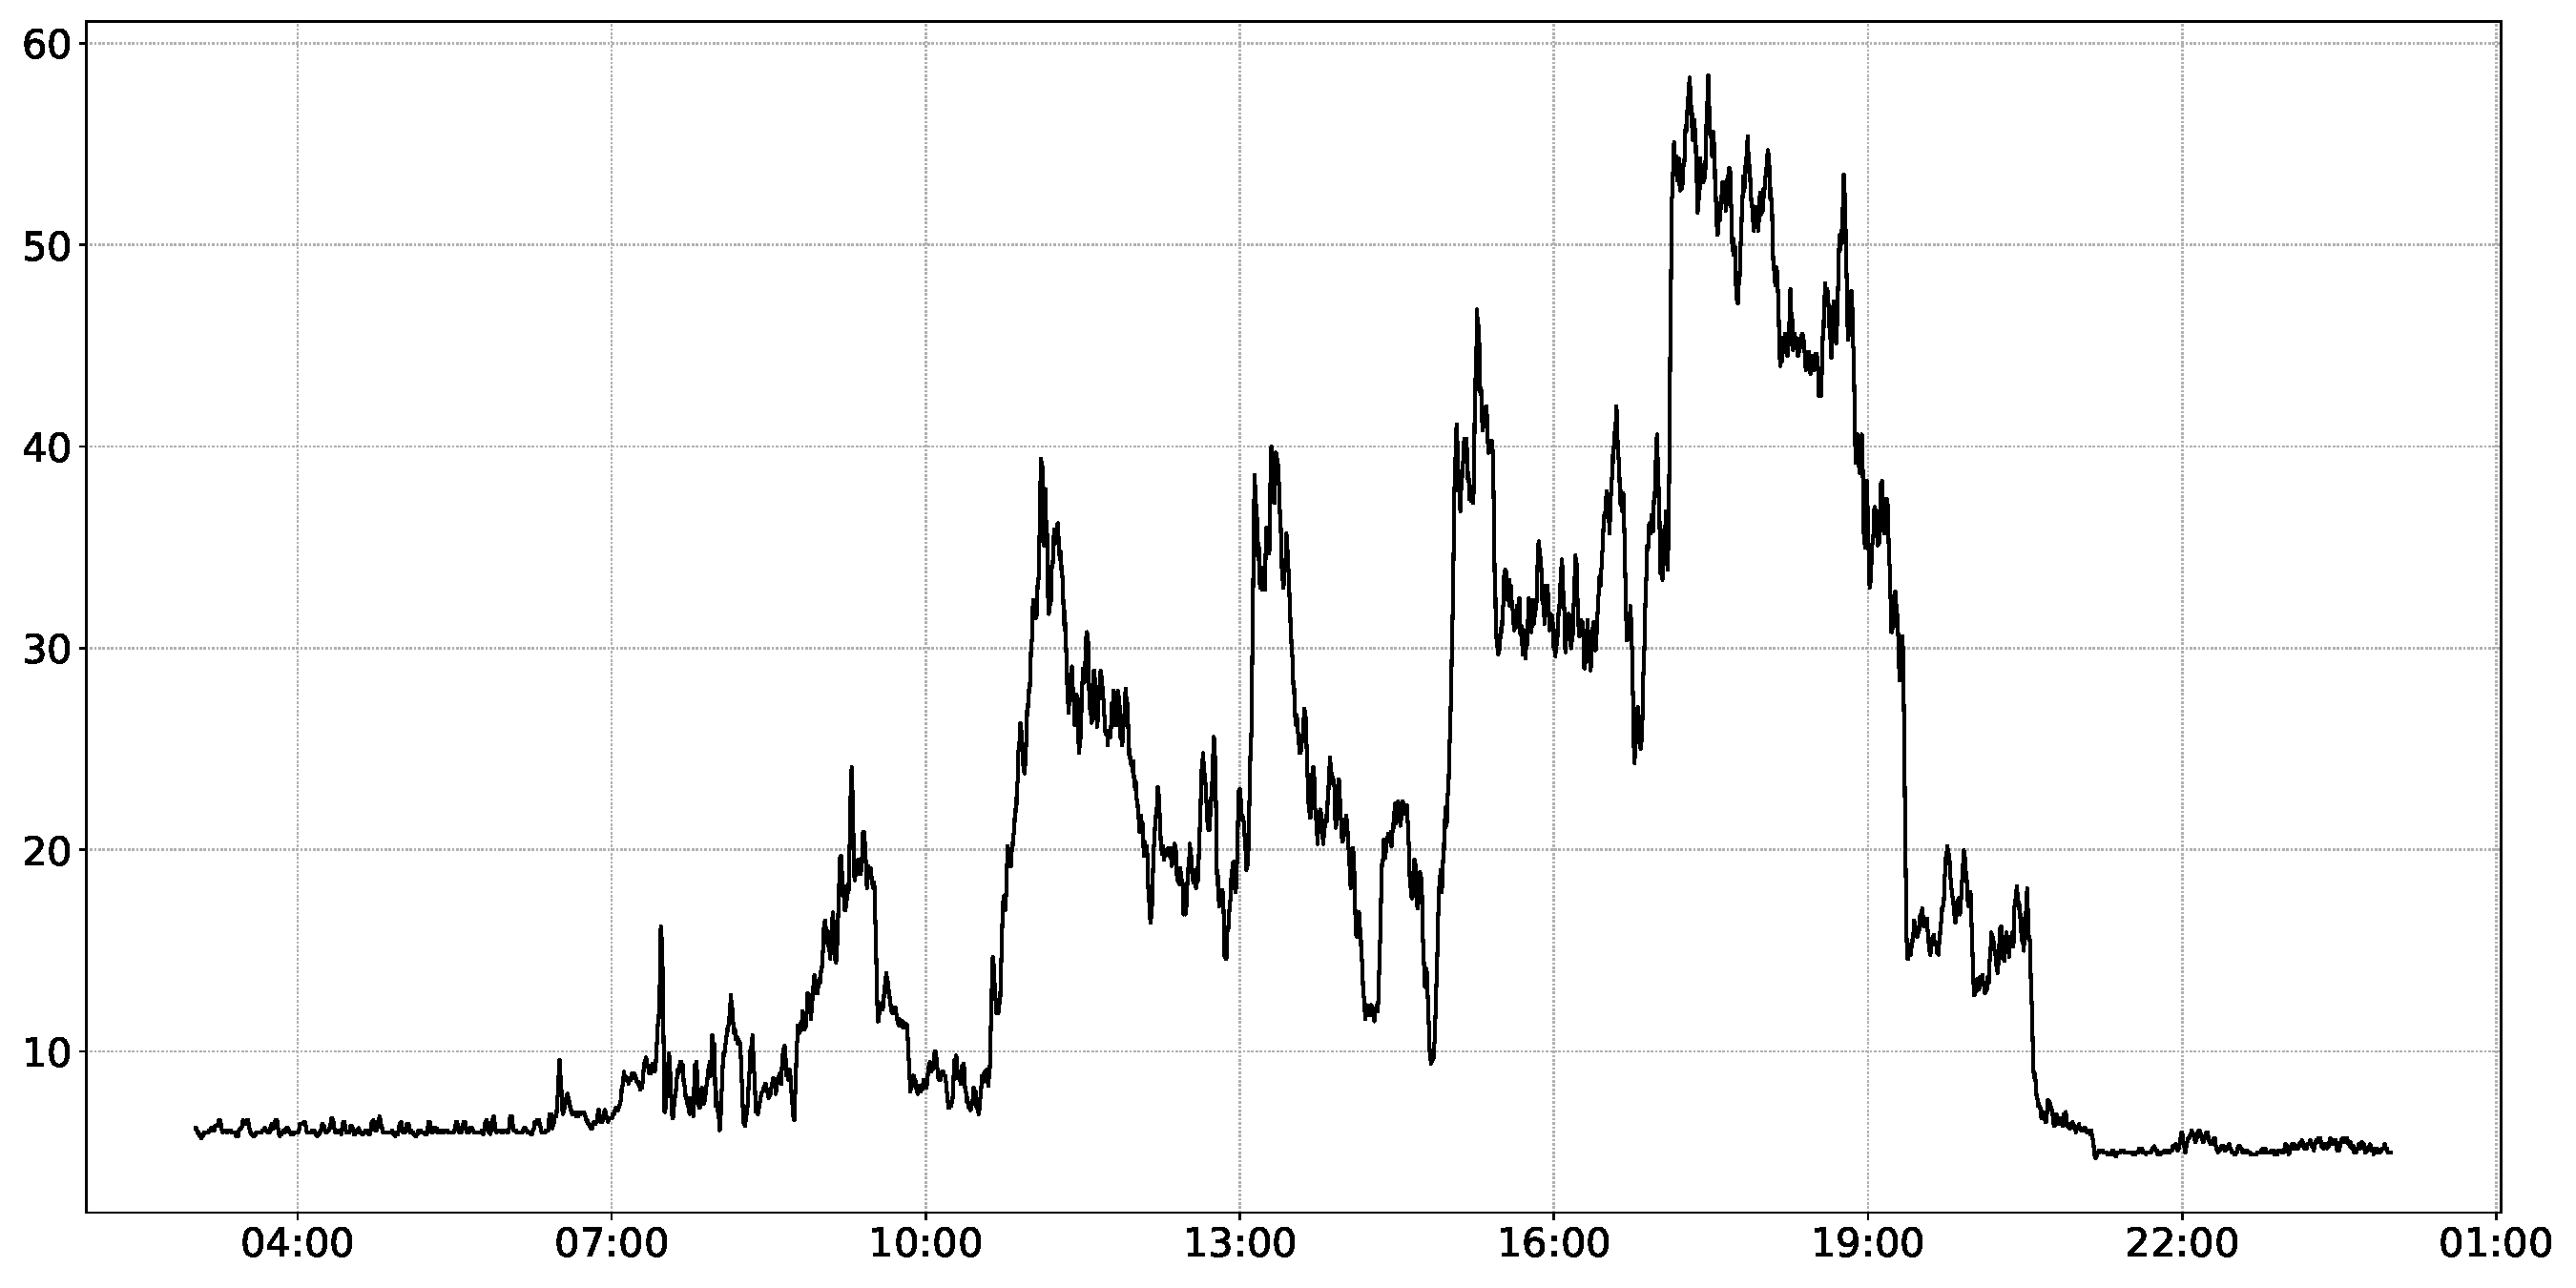
\includegraphics[width=0.8\linewidth]{dzien_wide.pdf}
        \caption{Sensor readings (number of unique BLE devices detected per 10-second scan) over the course of a representative weekday.}

    
    \label{fig:enter-label}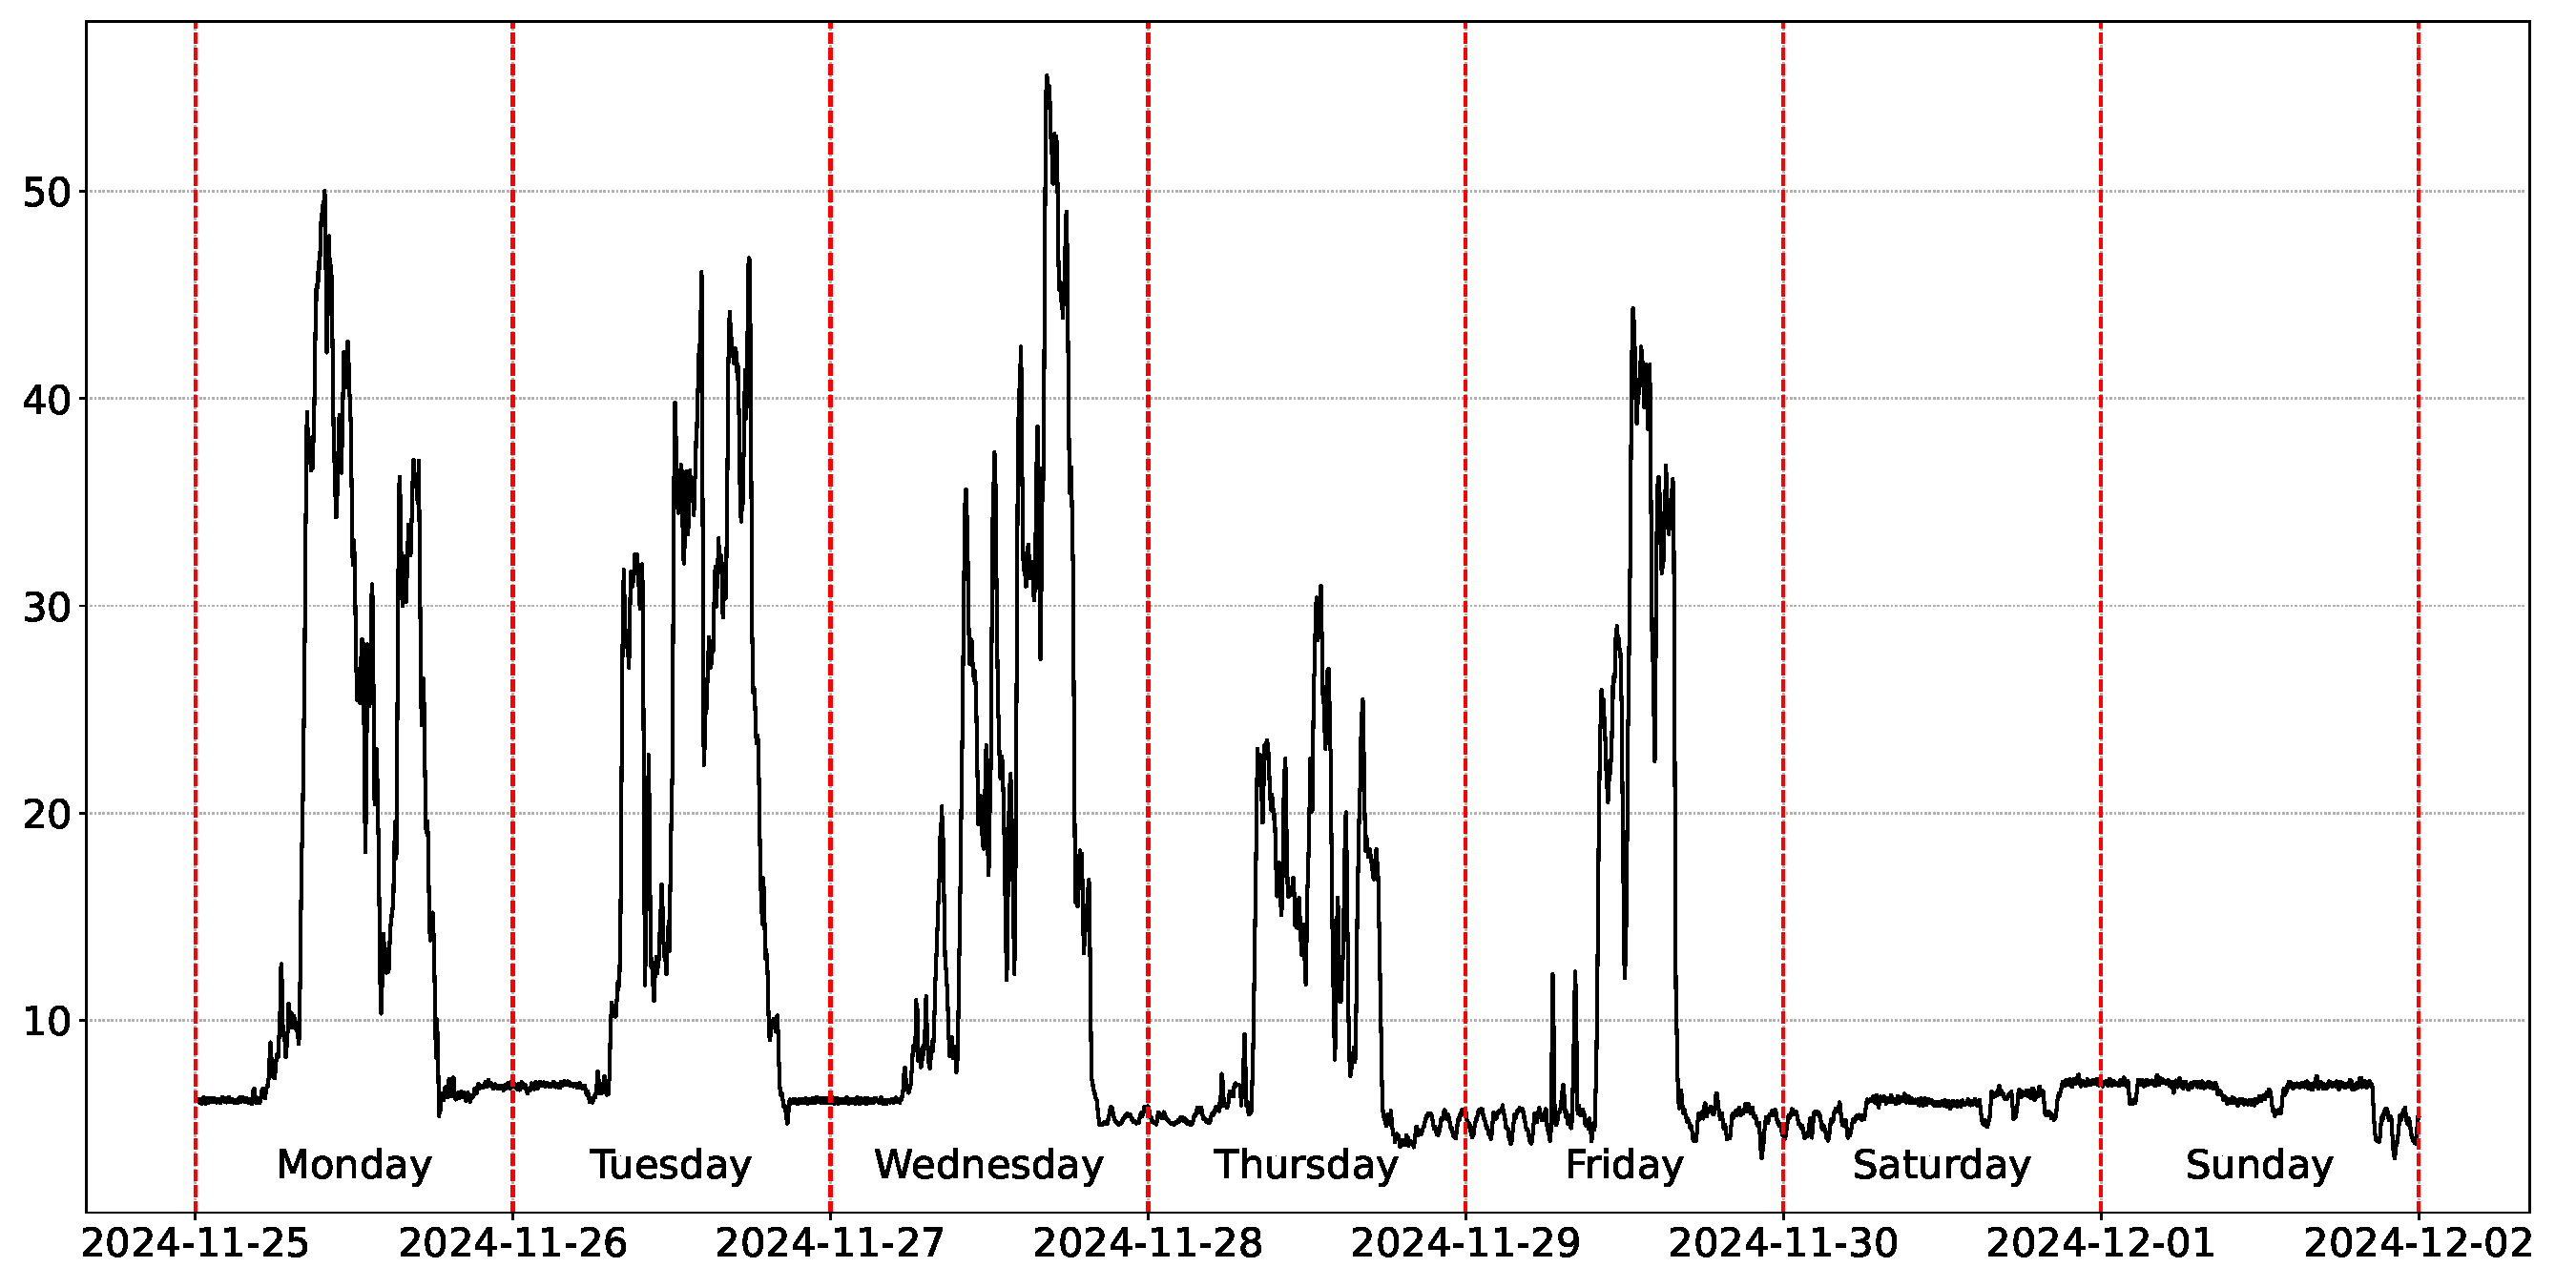
\includegraphics[width=0.8\linewidth]{foo_wide.pdf}
    \caption{Aggregated sensor readings (number of unique BLE devices) over the course of a full week, illustrating daily patterns and weekend lulls.}
    
\end{figure}

Our findings are based on a limited amount of data collected from a single sensor location and are intended to provide a preliminary indication of the system's capabilities.

Our initial analysis focuses on the time series data shown in Figures 1 and 2. The time series graph for this sensor (Fig. 1) shows clear
fluctuations in detected Bluetooth device counts over the course of a typical weekday. Notably, we observed that peaks in device counts correlate strongly
with the scheduled start and end times of classes in nearby classrooms. 
Specifically, we see a rapid increase in detected devices around the start of scheduled class hours (e.g., at the top of the hour when classes typically begin),
followed by a gradual decline during the class period. A subsequent peak occurs as students leave the classrooms at the end of the session; furthermore, during
periods when students are not present (night/weekends/holidays), we are able to observe the "baseline" reading of devices consistently in range of the sensor.
These preliminary results suggest that our system is effectively capturing the expected temporal patterns of occupancy within the monitored space. The ability
to discern these patterns, even with data from a single sensor, indicates the potential of our approach to provide valuable insights into real-time congestion
and space utilization. It is important to note that these findings are preliminary and based on a limited data set from a single sensor. More detailed analysis with data from larger deployments over a longer period is needed to validate these observations and draw more definitive conclusions.




\section{Broader Applications and Use Cases}
The principles and technology underpinning the BLE-based congestion monitoring system described in this paper extend to a wide array of applications beyond simple public space density estimation. The ability to passively and cost-effectively gather insights into human presence opens up opportunities across various sectors. This section outlines several key areas where such a system can provide substantial value:
\begin{enumerate}
    \item  Retail Environments-
    Stores can use BLE sensors to monitor foot traffic in aisles, optimize staffing during peak hours, and understand zone popularity and dwell times to enhance product placement strategies.

    \item  Smart Buildings-
    The system can be integrated into building management platforms to dynamically adjust lighting, HVAC, and access control based on real-time zone occupancy\cite{AlFuqaha_IoT}.

    \item  Event Management-
    Concerts, conferences, and sports venues can leverage congestion heatmaps derived from sensor data to manage crowd flow, reduce bottlenecks, and ensure safety compliance by monitoring zone capacities.

    \item  Urban Planning-
    Municipalities can deploy BLE sensors in public spaces, transport hubs, or parks to assess usage patterns of specific zones, inform infrastructure development, and prioritize maintenance schedules based on area occupancy.
\end{enumerate}


In these applications, the system provides valuable quantitative data on the presence and relative density of people within specific, sensor-defined areas. This information, while not tracking individuals, empowers data-driven decision-making for optimizing operations, resource allocation, and user/visitor experience.
The versatility of a low-cost, passive BLE sensing network, as demonstrated by the core congestion monitoring application, thus provides a foundational technology for a multitude of data-driven solutions aimed at creating more efficient, responsive, and user-centric environments.

\subsection{Challenges, Limitations, and Future Research Directions}
While our system demonstrates promising preliminary results for BLE-based congestion monitoring, it is important to recognize several limitations and challenges that influence its current performance and potential scalability:
\begin{itemize}
    \item Use of Locally Administered Addresses (LAA): As thoroughly documented by researchers \cite{Martin2017}, modern Bluetooth devices frequently randomize their MAC addresses using LAA schemes. While this enhances user privacy (as discussed in Section 3.6), it significantly complicates the process of consistently identifying unique devices across multiple scans or over extended periods. A key challenge is that a single device may be counted multiple times if it changes its MAC address within a short scan interval (e.g., our 10-second window), potentially leading to inflated congestion estimates in those specific instances.
    \item     Static Devices in Detection Range: As observed during threshold calibration (Section 3.4), a baseline of approximately 10 devices was consistently detected in laboratory L2.3, likely from fixed infrastructure. While this can be accounted for in location-specific calibration, changes in background device presence (e.g., adding or removing equipment) could impact accuracy if not recalibrated.
    \item     Device-Person Ratio Variability: The estimated 3:1 device-to-person ratio, based on informal surveys in an academic context, is an approximation. This ratio likely varies significantly depending on the environment (e.g., students with multiple devices vs. general public visitors) and demographics, impacting the direct translation of device counts to precise person counts.
    \item     Environmental Interference and Signal Propagation: BLE signal strength (RSSI) and detectability are influenced by physical obstacles such as walls and furniture, as well as by peaple absorbing RF signals. This can lead to fluctuating readings or reduced detection range even with a constant number of devices, particularly in complex or less controlled indoor environments.
    \item     Limited Sample Size and Validation for Initial Findings: The preliminary findings presented rely on data from a single sensor and calibration in a specific lab environment. Broader validation with more diverse deployments and real-time ground truth data (e.g., live headcounts or camera-assisted verification) is needed for robust system assessment
\end{itemize}









\subsection{Conclusion and Future Work}
 To address the identified challenges and further enhance the system's capabilities, future research will explore several key directions:
\begin{itemize}
    \item    Addressing LAA-Induced Counting Inaccuracies: Investigating and developing methods to better handle or mitigate the impact of randomized MAC addresses on count accuracy, particularly focusing on intra-scan address changes.

   \item  Multi-Sensor Deployments and Data Fusion: Expanding to multi-sensor deployments to improve coverage, provide spatial resolution of congestion, and potentially use techniques like trilateration (with RSSI, cautiously) or data fusion to enhance accuracy.

    \item Advanced Congestion Estimation Algorithms: Implementing machine learning approaches (e.g., time series forecasting, anomaly detection, adaptive thresholding) to dynamically infer congestion levels based on historical data, contextual patterns, and potentially real-time feedback.

    \item Cross-Verification with Other Sensor Modalities: Exploring the integration with other sensor types (e.g., Wi-Fi sniffers, thermal cameras – with careful privacy considerations) for data cross-verification and a more holistic understanding of occupancy.

    \item Refining Device-to-Person Ratio Estimation: Conducting more extensive and structured surveys across diverse environments and user groups to develop more accurate and context-aware models for the device-to-person ratio.

    \item Enhanced Visualization and Reporting: Developing more sophisticated visualization tools, such as interactive real-time heatmaps overlaid on digital maps, and automated statistical reporting capabilities
\end{itemize}
\begin{credits}
\end{credits}
%
% ---- Bibliography ----
%
% BibTeX users should specify bibliography style 'splncs04'.
% References will then be sorted and formatted in the correct style.
%
% \bibliographystyle{splncs04}
% \bibliography{mybibliography}
%
\begin{thebibliography}{8}
\bibitem{Espressif}
Espressif ESP32-C3 Datasheet.\\
\url{https://www.espressif.com/sites/default/files/documentation/esp32-c3\_datasheet\_en.pdf}\\ last accessed 30.06.2025.



\bibitem{Grafana}
Grafana Labs. "Grafana: The open observability platform."\\
\url{https://grafana.com/}\\
last accessed 30.06.2025

\bibitem{MQTT}
OASIS Standard. "MQTT Version 5.0."\\
\url{https://docs.oasis-open.org/mqtt/mqtt/v5.0/os/mqtt-v5.0-os.html}\\
last accessed 30.06.2025

\bibitem{Telegraf}
InfluxData. "Telegraf - The plugin-driven server agent for collecting \& reporting metrics."\\
\url{https://www.influxdata.com/time-series-platform/telegraf/}\\
last accessed 30.06.2025

\bibitem{Bluetooth}
Bluetooth SIG. "Bluetooth Core Specification, Version 5.3."\\
\url{https://www.bluetooth.com/specifications/specs/core-specification-5-3/}\\
last accessed 30.05.2025

\bibitem{Zafari_Localization}
Zafari, F., Gkelias, A., \& Leung, K. K. "A survey of indoor localization systems and technologies." *IEEE Communications Surveys \& Tutorials*, 21(3), 2568-2599 (2019).

\bibitem{AlFuqaha_IoT}
Al-Fuqaha, A., et al. "Internet of Things: A survey on enabling technologies, protocols, and applications." *IEEE Communications Surveys \& Tutorials*, 17(4), 2347-2376 (2015).

\bibitem{Martin2017}
Martin, E., et al.: A study of MAC address randomization in mobile devices and when it fails. In: Proceedings of the 16th Workshop on Privacy in the Electronic Society (WPES), pp. 1--12 (2017).
\end{thebibliography}

\end{document}
\end{document}
